\newcommand{\texCommand}[1]{\texttt{\textbackslash{#1}}}%

\newcommand{\exemplo}[1]{%
\vspace{\baselineskip}%
\noindent\fbox{\begin{minipage}{\textwidth}#1\end{minipage}}%
\\\vspace{\baselineskip}}%

\newcommand{\exemploVerbatim}[1]{%
\vspace{\baselineskip}%
\noindent\fbox{\begin{minipage}{\textwidth}%
#1\end{minipage}}%
\\\vspace{\baselineskip}}%
\label{cap:fundamentação}
\section{ROS} 
O ROS \cite{ros1} é um framework amplamente utilizado no desenvolvimento de sistemas robóticos que compõe um conjunto de bibliotecas, ferramentas e convenções que facilitam a criação de aplicações robóticas modulares e distribuídas. Por meio de uma arquitetura baseada em nós (nodes) e tópicos (topics), o ROS permite a comunicação entre diferentes componentes do sistema, promovendo a reutilização de código e a integração de diversos sensores e atuadores. 

No caso do \textit{ROS 2} \cite{ros2}, essa arquitetura foi reformulada para superar limitações da versão anterior, adotando o padrão \textit{DDS (Data Distribution Service)} como base para a comunicação entre processos. Essa mudança garante maior confiabilidade, escalabilidade e suporte a aplicações em tempo real, além de possibilitar o uso de políticas de Qualidade de Serviço (QoS) que permitem ajustar aspectos como latência, persistência e confiabilidade das mensagens. A comunicação no ROS 2 ocorre de forma totalmente distribuída, dispensando a presença de um nó mestre e favorecendo a robustez em sistemas heterogêneos. Nessa arquitetura, os nós permanecem como unidades computacionais fundamentais e podem publicar ou assinar mensagens em tópicos, realizar chamadas de serviços no modelo requisição-resposta, gerencia ciclo de vida ou ainda empregar ações para lidar com tarefas de longa duração. Adicionalmente, parâmetros podem ser configurados em tempo de execução, permitindo a adaptação dinâmica do comportamento de um nó, e a execução dessas interações é gerida por um mecanismo de execução denominado executor, responsável por organizar e disparar as funções de retorno de acordo com os eventos que ocorrem. Dessa forma, a arquitetura do ROS 2 fornece uma base flexível, modular e resiliente, capaz de atender às demandas crescentes da robótica moderna. Na figura \ref{fig:interface} visualiza as dinâmica arquitetural de um sistema em ROS.

\begin{figure}[H]
\centering
   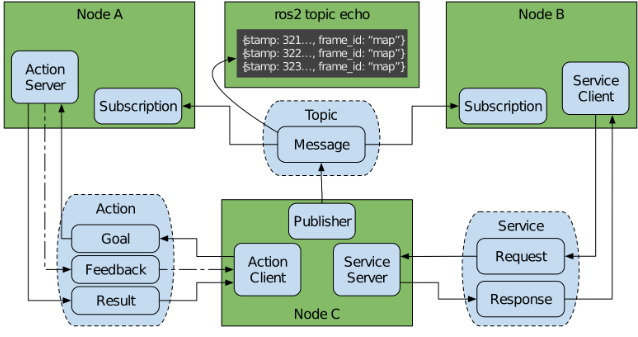
\includegraphics[width=1\textwidth]{img/ros2/ros2figura.png}
    \caption{figura do artigo \cite{ros2} mostrando as interfaces do ROS}
    \label{fig:interface}
\end{figure}

\subsubsection{Diferenças entre ROS 1 e ROS 2}

O ROS 1 consolidou-se como um dos principais ambientes de pesquisa em robótica, porém foi projetado 
com foco acadêmico e com menos suporte para requisitos de larga escala ou uso em ambientes industriais. Algumas de 
suas limitações incluem a ausência de suporte nativo para sistemas embarcados de tempo real, dificuldades na comunicação 
entre múltiplos robôs em rede distribuída, e problemas de segurança e escalabilidade.

O ROS 2 surgiu como resposta a essas limitações. Construído sobre o \textit{Data Distribution Service} (DDS) \cite{dds_spec}, um padrão 
de comunicação usado em sistemas críticos, o ROS 2 introduz melhorias significativas, tais como: (i) Suporte a comunicação em tempo real; (ii) Melhor gerenciamento de qualidade de serviço (QoS); (iii) Arquitetura projetada para sistemas distribuídos e multi-robô; (iv) Maior portabilidade, incluindo suporte a sistemas embarcados; (v) Recursos de segurança integrados (criptografia e autenticação).

\section{Recuperação de \textit{Ground Truth} Comportamental}

A recuperação de \textit{ground truth} em sistemas
legados é abordada por Garcia et al.~\cite{GarciaKMD12}
no contexto da recuperação arquitetural de software.
Os autores propõem um \textit{framework} para obter
uma representação arquitetural de referência,
combinando técnicas de recuperação, informações
sobre o sistema e conhecimento especializado.

O processo parte de uma recuperação arquitetural
inicial, produzida por técnicas genéricas de
recuperação (\textit{generic recovery techniques}),
que identificam e agrupam entidades de implementação
em componentes arquiteturais candidatos.
Essa representação é examinada considerando
informações de domínio e aplicação, além de
princípios relacionados à organização e ao
contexto do sistema.

A recuperação inicial é posteriormente refinada
por meio de um processo de certificação, no qual
um especialista com conhecimento aprofundado
do sistema (\textit{certifier}) avalia a adequação
da representação recuperada. Esse processo pode
envolver modificações nos componentes e nas
relações identificadas, buscando estabelecer
uma representação arquitetural considerada
autoritativa para o sistema investigado.

A recuperação de requisitos de sistemas legados
é investigada, sob outra perspectiva, por
Silva~\cite{TARCILArecreq}, que examina os
processos AMBOLS e CelLEST. Essas abordagens
buscam recuperar requisitos funcionais a partir
da observação das interações entre usuários
e sistemas existentes, utilizando, respectivamente,
conhecimento do domínio e modelagem comportamental,
ou a identificação de padrões de interação.

O estudo destaca a importância do conhecimento
dos usuários na interpretação das funcionalidades
recuperadas e na avaliação de sua correspondência
com o sistema existente. Diferentemente da
recuperação arquitetural de Garcia et al.,
seu objeto de investigação são os requisitos
funcionais, e não a construção de uma representação
arquitetural de referência.


\section{Compreensão de Programas}

A compreensão de um sistema de software existente é um pré-requisito para necessário para o processo de recuperação de \textit{ground truth} proposto por Garcia et al. que exige que o \textit{recoverer} reúna informações de domínio e de aplicação e extraia informações a nível de implementação antes de interpretar o sistema \cite{GarciaKMD12}. A documentação disponível do sistema pode descrever componentes esperados, conectores, funcionalidades e informações do contexto do sistema, enquanto os artefatos de implementação fornecem evidências sobre relações entre entidades no nível do código.

A \textit{compreensão de programas} diz respeito ao processo pelo qual desenvolvedores adquirem conhecimento sobre um sistema de software existente e constroem representações mentais que relacionam detalhes de implementação a conceitos funcionais e de domínio de nível mais alto~\cite{von,Siegmund}.

Os modelos clássicos de compreensão caracterizam processos como \textit{top-down} e \textit{bottom-up}. Na compreensão \textit{top-down}, o conhecimento prévio sobre o domínio da aplicação sustenta hipóteses sobre o propósito geral e a organização do programa, que são constantemente refinadas em direção aos elementos no nível de implementação. Na compreensão \textit{bottom-up}, os desenvolvedores começam pelas instruções do programa e pelas estruturas de implementação, agrupando-as em abstrações de nível superior~\cite{von,Siegmund}. Na prática, a compreensão pode alternar entre esses processos à medida que novas evidências são obtidas.

Von Mayrhauser e Vans~\cite{von} integram essas perspectivas por meio do \textit{Integrated Metamodel} de compreensão de programas. O metamodelo combina um modelo \textit{top-down}, um modelo de programa, um modelo de situação e uma base de conhecimento compartilhado. O modelo de programa representa conhecimento orientado à implementação, construído a partir do código e de informações de fluxo de controle, enquanto o modelo situacional relaciona entidades de implementação a conhecimentos sobre fluxo de dados, funcionalidades e domínio. A base de conhecimento norteia o processo de compreensão ao disponibilizar conhecimentos previamente adquiridos sobre programação, domínio e sistema.

Essa perspectiva fornece a fundamentação teórica para a etapa de Compreensão de Programas adotada na metodologia. O conhecimento existente sobre o sistema legado pode orientar a investigação inicial, enquanto as evidências obtidas de sua implementação e execução podem ser utilizadas para refinar ou reconsiderar essa compreensão. As visões estáticas e dinâmicas são, portanto, tratadas como evidências externas que apoiam o processo de compreensão.

O uso de representações visuais também é consistente com a literatura mais ampla de visualização da arquitetura de software. Shahin et al.~\cite{Shahin2014} identificam técnicas de visualização destinadas a apoiar a compreensão de características arquiteturais estáticas e comportamentais, bem como a rastreabilidade entre entidades arquiteturais e artefatos de software.

\section{Behavior Driven Development (BDD)}

    O \textit{Behavior-Driven Development} (BDD) permite expressar requisitos comportamentais como cenários estruturados, baseados em exemplos. Farooq et al.~\cite{Farooq2023BDD} revisam aplicações de BDD e descrevem um fluxo de desenvolvimento no qual requisitos ou histórias de usuário são elaborados na forma de cenários comportamentais.

    A qualidade dessas especificações também depende de seu vocabulário de domínio, da reutilização de passos e do nível de abstração, conforme investigado por Binamungu et al.~\cite{Binamungu}.
    Essa é abordagem visa diminuir a lacuna entre partes técnicas e não técnicas, definindo o comportamento do sistema em linguagem clara e padronizada. A sintaxe usada segue o padrão \texttt{Given-When-Then} (Dado-Quando-Então).
    
    A \textit{ground-truth} foi elaborada como um conjunto de cenários, expressos em linguagem natural, que formalizam os requisitos do sistema, seguindo a sintaxe BDD:

\begin{lstlisting}[language=Gherkin, , basicstyle=\small\ttfamily]
Scenario: [scenario description]
    Given that [...]
    When I [...]
    And I [...]
    Then [...]
\end{lstlisting} 

No contexto da robótica, onde sistemas complexos operam em ambientes imprevisíveis e executam comportamentos elaborados, o BDD é uma abordagem alternativa para analisar e gerenciar requisitos, além de introduzir automação na verificação e validação. Os livros de regras de competições robóticas e benchmarks, por exemplo, são fontes públicas de requisitos e critérios de aceitação para avaliar o desempenho de robôs, descrevendo cenários de teste e a avaliação em si, como descrito no artigo \cite{BDDStudy}.


No contexto dessa sintaxe, o passo \textit{Given} descreve as condições iniciais ou o estado do sistema antes da execução do comportamento a ser verificado, representando o cenário de preparação para o teste. O passo \textit{When} indica a ação ou evento que desencadeia o comportamento esperado, funcionando como o gatilho principal que deve alterar o estado do sistema. O uso do \textit{And} permite a inclusão de múltiplas condições ou ações adicionais nos blocos \textit{Given}, \textit{When}, \textit{Then}, possibilitando a modelagem de cenários mais complexos sem perda de clareza. Finalmente, o passo \textit{Then} especifica o resultado esperado após a execução da ação, descrevendo de forma objetiva a saída ou estado final do sistema que será utilizado como critério de verificação do teste. Dessa maneira, a sintaxe \texttt{Given-When-Then} garante que cada cenário expresse claramente o contexto, o estímulo e a resposta esperada, estabelecendo uma ponte entre a especificação de requisitos e sua validação prática.

Nguyen et al.~\cite{Nguyen2025BDD} ampliam essa linha de investigação ao propor uma abordagem baseada em modelos para a especificação e execução automatizada de testes de aceitação em sistemas robóticos. Os autores estendem a representação de cenários BDD para incorporar restrições temporais, informações específicas do domínio e relações entre comportamentos. A abordagem utiliza modelos estruturados para gerar cenários Gherkin executáveis e avaliá-los em um ambiente de simulação robótica.

O estudo também identifica desafios na automação dos testes, especialmente na coordenação entre a execução do comportamento, a coleta das informações necessárias e a avaliação dos critérios de aceitação. Esses desafios evidenciam que a especificação de um comportamento em BDD não assegura, isoladamente, sua verificação então é necessário implementar mecanismos de observação e asserções compatíveis com os critérios estabelecidos.


\section{Testes de Caracterização e Oráculos de Teste}

A manutenção e a evolução de sistemas legados necessitam da compreensão de comportamentos exigidos que não necessariamente correspondem à implementação existente. Nesse contexto, Feathers~\cite{Feathers2004} discute os testes de caracterização como uma estratégia para investigar e registrar o comportamento apresentado pelo código antes de sua modificação.

Essa caracterização permite documentar respostas e dependências existentes, mas não demonstra, necessariamente, que os resultados observados sejam corretos. O comportamento legado pode incluir defeitos ou decisões de implementação que não correspondem às expectativas atuais do sistema.

A determinação da correção dos resultados está relacionada ao problema do oráculo de teste (\textit{test oracle problem}), investigado por Barr et al.~\cite{Barr2015}. Um oráculo de teste consiste em um mecanismo ou procedimento que permite avaliar se determinado comportamento observado corresponde ao comportamento esperado. Os autores discutem diferentes fontes de informação para estabelecer oráculos, incluindo especificações, contratos, modelos e conhecimento humano sobre o domínio da aplicação.

Quando os requisitos estão disponíveis, seus critérios de aceitação podem fornecer expectativas para a verificação do comportamento. Entretanto, essas expectativas precisam ser representadas por asserções executáveis capazes de observar as propriedades pretendidas. Uma asserção que verifica apenas parte do comportamento especificado pode produzir um resultado de aprovação sem demonstrar a satisfação integral do requisito.

Desse modo, a caracterização do comportamento existente e a verificação de sua conformidade com requisitos são atividades complementares. A primeira fornece evidências sobre o funcionamento observado da implementação, enquanto a segunda utiliza oráculos para interpretar essas observações em relação ao comportamento esperado. Essa distinção é relevante para a evolução de sistemas legados, pois permite diferenciar comportamentos que devem ser preservados, discrepâncias conhecidas e observações cuja adequação permanece inconclusiva.

\section{Migração e Transformação de Software}

A migração de software envolve a transformação de sistemas existentes para novos ambientes podendo abranger alterações nas linguagens de programação, plataformas, interfaces e arquiteturas. Bragagnolo et al.~\cite{BragagnoloMigration} apresentam um framework teórico para a modernização de software como a abordagem \textit{white-box}, que examina a implementação interna do legado.

Os autores também discutem o modelo de processo \textit{Horseshoe}, associado à migração de um sistema existente para uma nova implementação. Esse processo compreende cinco atividades:

\begin{enumerate}
    \item \textbf{Planejamento:} delimitar os objetivos, o escopo e as prioridades da migração, considerando sua viabilidade, custos e riscos.
    \item \textbf{Compreensão do sistema de origem:} recuperar conhecimento sobre o sistema legado por meio da documentação, inspeção do código e técnicas de engenharia reversa. Essa atividade permite compreender sua organização, funcionalidades e dependências.
    \item \textbf{Compreensão do sistema de destino:} identificar as características, restrições e comportamentos esperados da nova implementação, considerando também suas interações com o ambiente.
    \item \textbf{Transformação do conhecimento:} utilizar o conhecimento adquirido sobre os dois sistemas para determinar como as estruturas e funcionalidades existentes serão adaptadas ou reorganizadas conforme as características do destino.
    \item \textbf{Produção do sistema de destino:} aplicar as transformações identificadas para construir a nova implementação, por procedimentos manuais, semiautomáticos ou automáticos.
\end{enumerate}

Nesse modelo, a compreensão das implementações de origem e destino fundamenta as decisões de transformação, que, por sua vez, orientam a produção do sistema migrado.

No domínio dos sistemas ciberfísicos, a migração também envolve desafios relacionados à integração de componentes, à comunicação distribuída e às restrições operacionais. Foehr et al. \cite{Foehr2017} discutem a transformação de arquiteturas tradicionais de automação para arquiteturas distribuídas, destacando estratégias incrementais de migração e a necessidade de considerar dependências entre os elementos do sistema. Ressaltam ainda que a migração de sistemas ciberfísicos apresenta desafios adicionais relacionados aos requisitos temporais e operacionais.
%esse artigo pode ajudar a justificar a análise de realizações comportamentais
 Buchgeher et al. \cite{BUCHGEHER2022276} apresentam um estudo de migração de sistemas ciberfísicos industriais para OPC UA, no qual técnicas de análise estática são utilizadas para identificar elementos da implementação legada, como variáveis acessíveis externamente, funções invocáveis e instâncias de variáveis. Essas informações são utilizadas para construir modelos de informação que orientam a geração de componentes, documentação e testes de integração. Os autores também identificam limitações na geração de testes envolvendo interações complexas entre métodos e variáveis, que exigem informações adicionais sobre a implementação.

A transformação da implementação também levanta questões relacionadas à preservação do comportamento do sistema. AlOmar et al.~\cite{AlOmar2021} investigam abordagens de preservação comportamental no contexto da refatoração de software, incluindo técnicas de análise estática, análise dinâmica e verificação formal.

Embora a refatoração seja caracterizada pela modificação da estrutura interna sem alterar o comportamento externo, a migração entre plataformas pode envolver mudanças mais abrangentes, incluindo a substituição de mecanismos de comunicação, execução e organização dos componentes. O planejamento de transformações em sistemas legados depende do conhecimento sobre a implementação de origem e das características do ambiente de destino. Na perspectiva de migração \textit{white-box} discutida por ~\cite{BragagnoloMigration}, a compreensão das entidades e das relações existentes no sistema fornece informações para examinar as mudanças necessárias à sua modernização. Essas transformações podem envolver adaptações tecnológicas, reorganização de responsabilidades e modificações nas interfaces entre componentes.

\section{Rastreabilidade entre Comportamentos e Implementação}

A identificação das entidades de implementação associadas a determinadas funcionalidades constitui um problema investigado pela área de localização de funcionalidades (\textit{feature location}). Dit et al.~\cite{Dit2013} apresentam diferentes abordagens para a localização de funcionalidades no código-fonte, incluindo técnicas baseadas em análise estática e dinâmica. A identificação dessas entidades auxilia a compreensão de programas e fornece informações para atividades de manutenção e evolução de software.

Em sistemas baseados em ROS, as relações entre componentes também podem ser examinadas por meio de suas interfaces de comunicação. O grafo computacional, visualizado por ferramentas como \texttt{rqt\_graph}, apresenta nós, tópicos e relações entre publicadores e assinantes. Essa representação permite investigar a organização da comunicação, mas não demonstra, isoladamente, quais mensagens são transmitidas durante a execução de determinado comportamento. A observação do fluxo de dados pode ser complementada pelos mecanismos disponíveis na interface de linha de comando do ROS (\texttt{ROS CLI}).

A interpretação dessas relações, em conjunto com a inspeção do código-fonte, dos grafos de chamadas e dos arquivos de inicialização, permite investigar as entidades de implementação associadas aos comportamentos do sistema e caracterizar suas respectivas responsabilidades.

\section{Testes de Regressão e Preservação Comportamental}

Os testes de regressão buscam identificar alterações não intencionais no comportamento do software após modificações em sua implementação. No contexto da evolução de sistemas legados, esses testes permitem investigar se funcionalidades anteriormente verificadas continuam satisfazendo os requisitos estabelecidos após a realização de transformações.

A preservação de comportamento também constitui uma preocupação central na refatoração de software. AlOmar et al.~\cite{AlOmar2021} investigam abordagens utilizadas para avaliar a preservação comportamental durante operações de refatoração. Entretanto, migrações entre plataformas podem envolver transformações mais abrangentes, incluindo mudanças de linguagem, interfaces e mecanismos de execução.

A preservação comportamental pode envolver a comparação entre diferentes implementações. Essa perspectiva relaciona-se ao teste diferencial, discutido por McKeeman~\cite{McKeeman1998}, no qual respostas obtidas a partir de entradas comparáveis são confrontadas. Contudo, a concordância entre implementações não demonstra necessariamente a satisfação dos requisitos, pois ambas podem apresentar comportamentos incorretos.

Assim, a utilização de testes de regressão na migração de software requer considerar os critérios de aceitação, os estímulos aplicados, as condições de execução e os resultados efetivamente observados.


